\documentclass[review]{elsarticle}
\usepackage[spanish]{babel}
\usepackage{graphicx}
\usepackage{subfig}
\usepackage{lineno,hyperref}
\usepackage{natbib}
\setcitestyle{numbers,sort&compress}
\usepackage{float}
\usepackage{footmisc}
\usepackage{adjustbox}
\usepackage{tikz}
\usepackage{listing}
\usepackage{pythonhighlight}
\usepackage{rotating}
\usepackage{array,booktabs,makecell}
\usepackage{amssymb}
\modulolinenumbers[5]

%\journal{Journal of \LaTeX\ Templates}


\newenvironment{abstracts}
 {\global\setbox\absbox=\vbox\bgroup
    \hsize=\textwidth
    \linespread{1}\selectfont}
 {\vspace{-\bigskipamount}\egroup}
\renewenvironment{abstract}[1][]
 {\if\relax\detokenize{#1}\relax\else\selectlanguage{#1}\fi
  \noindent\textbf{\abstractname}\par\medskip\noindent\ignorespaces}
 {\par\bigskip}
 
 
\let\today\relax
\makeatletter
\def\ps@pprintTitle{%
    \let\@oddhead\@empty
    \let\@evenhead\@empty
    \def\@oddfoot{\footnotesize\itshape
         {} \hfill\today}%
    \let\@evenfoot\@oddfoot
    }
\makeatother
%%%%%%%%%%%%%%%%%%%%%%%
%% Elsevier bibliography styles
%%%%%%%%%%%%%%%%%%%%%%%
%% To change the style, put a % in front of the second line of the current style and
%% remove the % from the second line of the style you would like to use.
%%%%%%%%%%%%%%%%%%%%%%%

%% Numbered
%\bibliographystyle{model1-num-names}

%% Numbered without titles
%\bibliographystyle{model1a-num-names}

%% Harvard
%\bibliographystyle{model2-names.bst}\biboptions{authoryear}

%% Vancouver numbered
%\usepackage{numcompress}\bibliographystyle{model3-num-names}

%% Vancouver name/year
%\usepackage{numcompress}\bibliographystyle{model4-names}\biboptions{authoryear}

%% APA style
%\bibliographystyle{model5-names}\biboptions{authoryear}

%% AMA style
%\usepackage{numcompress}\bibliographystyle{model6-num-names}

%% `Elsevier LaTeX' style
\bibliographystyle{mighelnat}
%%%%%%%%%%%%%%%%%%%%%%%

\begin{document}

\begin{frontmatter}

\title{Inventarios forestales a través del procesamiento de imágenes}


\author{José Angel Ramírez Cantú}
\author{Satu Elisa Schaeffer}

\address{San Nicolás de los Garza, Nuevo León, México}

\begin{abstracts}
\begin{abstract}[spanish]
El impacto de la visión computacional en distintas áreas tiene un impacto positivo dando como resultado el poder resolver problemas de sectores diferentes a los de la tecnología. Es por eso que este trabajo propone utilizar la visión computacional en conjunto con el aprendizaje máquina para automatizar la clasificación de especies arbóreas y generación de inventarios forestales con el fin de reemplazar a las técnicas tradicionales que se utilizan en el sector forestal.
\end{abstract}

\textit{Palabras clave: } Procesamiento de imágenes, Aprendizaje máquina, Inteligencia artificial, Visión Computacional, Inventarios forestales.
\vspace*{0.5cm}
\end{abstracts}


\end{frontmatter}

\section{Introducción}

Este trabajo explica el funcionamiento de la solución propuesta para generar inventarios forestales utilizando el procesamiento de imágenes para la generación de inventarios forestales. Dicha solución consta de seis fases en las que se las que hace uso de muestras generadas a partir del recorrido de un dron en la zona del Cilantrillo y Trinidad (véanse las figuras \ref{Zona-cilantrillo} y \ref{Zona-trinidad} de la página \pageref{Zona-trinidad}). 

%%Duda #1, puedo referirme a las figuras de la misma página en una misma frase?

Aunque ya existen algunas software de computadora que ya tienen la facultad de poder detectar objetos, hay pocas soluciones que vayan totalmente enfocadas a generar inventarios forestales utilizando haciendo uso de tecnologías innovadoras que necesiten la menor interacción posible con el usuario que necesite generar un inventario forestal.
\clearpage

\begin{figure}[h!]
  \centering
\begin{tabular}{@{}ccc@{}}
\subfloat[Estatal]{\includegraphics[width=0.30\textwidth]{Lejos_C}} & 
\subfloat[Municipal]{\includegraphics[width=0.30\textwidth]{Medio_C}} &
\subfloat[Local]{\includegraphics[width=0.30\textwidth]{Cerca_C}}
  \end{tabular}
  \caption[Mapa de Cilantrillo]{El Cilantrillo, Montemorelos, Nuevo León (25.3523418, -100.3463186).}
   \label{Zona-cilantrillo}
\end{figure}

\begin{figure}[h!]
  \centering
\begin{tabular}{@{}ccc@{}}
\subfloat[Estatal]{\includegraphics[width=0.30\textwidth]{Lejos_t}} & 
\subfloat[Municipal]{\includegraphics[width=0.30\textwidth]{Medio_t}} &
\subfloat[Local]{\includegraphics[width=0.30\textwidth]{Cerca_t}}
  \end{tabular}
  \caption[Mapa de Trinidad.]{La Trinidad, Santiago, Nuevo León (25.225939, -100.1431609).}
  \label{Zona-trinidad}
\end{figure}

El objetivo de este trabajo es demostrar que la solución propuesta puede reducir tiempos a la hora de procesar las muestras recolectadas por el recorrido de un dron e identificar por sí misma, cada especie presente en las muestras recolectadas haciendo uso del procesamiento de imágenes. Otro de los objetivos es extraer la información de cada especie con el fin de generar un modelo a partir de la información recolectada en las especies de arboles definidas.\\

El artículo está divido en seis secciones, la sección 2 define los conceptos clave para el entendimiento del artículo, la sección 3 se presenta los artículos relacionados al presente trabajo y su diferencia, la sección 4 detalla la solución propuesta así como su metodología, la sección 5 se expone los resultados que apoyan a la hipótesis planteada  y los experimentos que permiten reafirmar la hipótesis inicial, finalmente la sección 6 presenta las conclusiones del artículo desarrollado y la contribución del presente artículo.

\section{Antecedentes}
La \emph{inteligencia artificial}\footnote{Ciencia encargada de desarrollar algoritmos capaces de imitar capacidades humanas} es una de las tecnologías que más ha acaparado la atención no sólo de las personas, sino también de las compañías que la utilizan con distintos fines, tanto cotidianos como industriales. Sin embargo, el porque de utilizarlas no sólo es con el fin de reemplazar las capacidades de un ser humano, sino que buscan facilitar las acciones con las que interactúa cada persona. En el caso del artículo se detalla como es que se busca utilizar la técnica de  \emph{procesamiento de imágenes}\footnote{Su función es capturar y procesar por medio de imágenes las información más relevante} para trabajar en conjunto con el \emph{aprendizaje máquina}\footnote{Campo de la inteligencia artificial que desarrolla algoritmos capaces de aprender por medio de información.} en el análisis de zonas forestales haciendo uso de \emph{clasificación de imágenes}\footnote{Es una técnica del aprendizaje máquina que consiste en identificar un objeto por medio de propiedades o características propias de un elemento.}.\\

El procesamiento de imágenes puede enfocarse en la búsqueda de un elemento en particular, por lo que permitiría reducir el tiempo que se invierte en clasificar individualmente cada especie de árbol y podría, paralelamente, identificar cada especie presente  a lo largo de un sector forestal no centrándose únicamente en una sola especie. Cabe destacar que el procesamiento de imágenes no sería posible sin la intervención de la \emph{visión computacional}\footnote{Técnica de la inteligencia artificial que intenta emular la capacidad visual de los humanos.} la cual es la que permitiría el detectar automáticamente cada especie en la solución propuesta.\\

%duda 2, puedo citar a alguien en un footnote?
En el caso de los \emph{inventarios forestales}\footnote{\citet{rf9} lo define como sistemas de recolección de características del área sobre el que se trabaja}, se va utilizar el procesamiento de imágenes para analizar las características de \textit{forma, color, bordes, textura} en las muestras, posteriormente el aprendizaje máquina tendrá que establecer en un modelo de información el análisis obtenido a partir de las características previamente mencionadas.

\subsection{Antecedentes históricos}
El procesamiento de imágenes surge en el año 1920 de los primeros intentos de transmisión de imágenes por medio de un cable transatlántico usando códigos telegráficos, permitiendo la codificación de una imagen en cinco niveles de gris para posteriormente, en 1929, el ya mencionado sistema de transmisión permitía codificar a quince niveles de gris, a su vez, este sistema redujo el tiempo de transmisión de imágenes a quince minutos \citep{rf4}.\\

El aprendizaje máquina surge a principios del año 1990 como un proceso para la extracción de información y modelos de predicción, esto último fue bastante utilizado por los sectores bancarios, que eran los que mayormente le sacaban un provecho a la hora de tomar decisiones \citep{rf5}.\\ 

La visión computacional llevaba bastante más tiempo que había sido desarrollada, pero no empleada; y es que en el año 1960 es cuando la inteligencia artificial apenas se estaba desarrollando y fue cuando se planteo el como es que una computadora iba a razonar como lo haría una persona. Los problemas recaen sobre factores de innovación y procesamiento de imágenes automático \citep{rf6}.

\subsection{Descriptores de características globales}
Existen dos tipos de características utilizados en el presente trabajo, las características globales que son las que pueden percibirse fácilmente (color, forma, textura) y las características locales, que cuantifican globalmente una imagen, estas últimas son necesarias son necesarias para determinar que descriptor de características es el mejor para describir los puntos de interés o cierta región de una imagen.
\clearpage

\subsubsection{Color}
La característica de clasificación de color hace uso del \emph{histograma de color}\footnote{Cantidad de pixeles en listas de rangos de colores presentes en una imagen.} y por medio de gráficas, determinar la intensidad de la distribución del valor de un \emph{pixel}\footnote{Es la unidad básica más pequeña de las imágenes.}.

\begin{figure}[h!]
  \centering
\begin{tabular}{@{}ccc@{}}
\subfloat[Muestra utilizada]{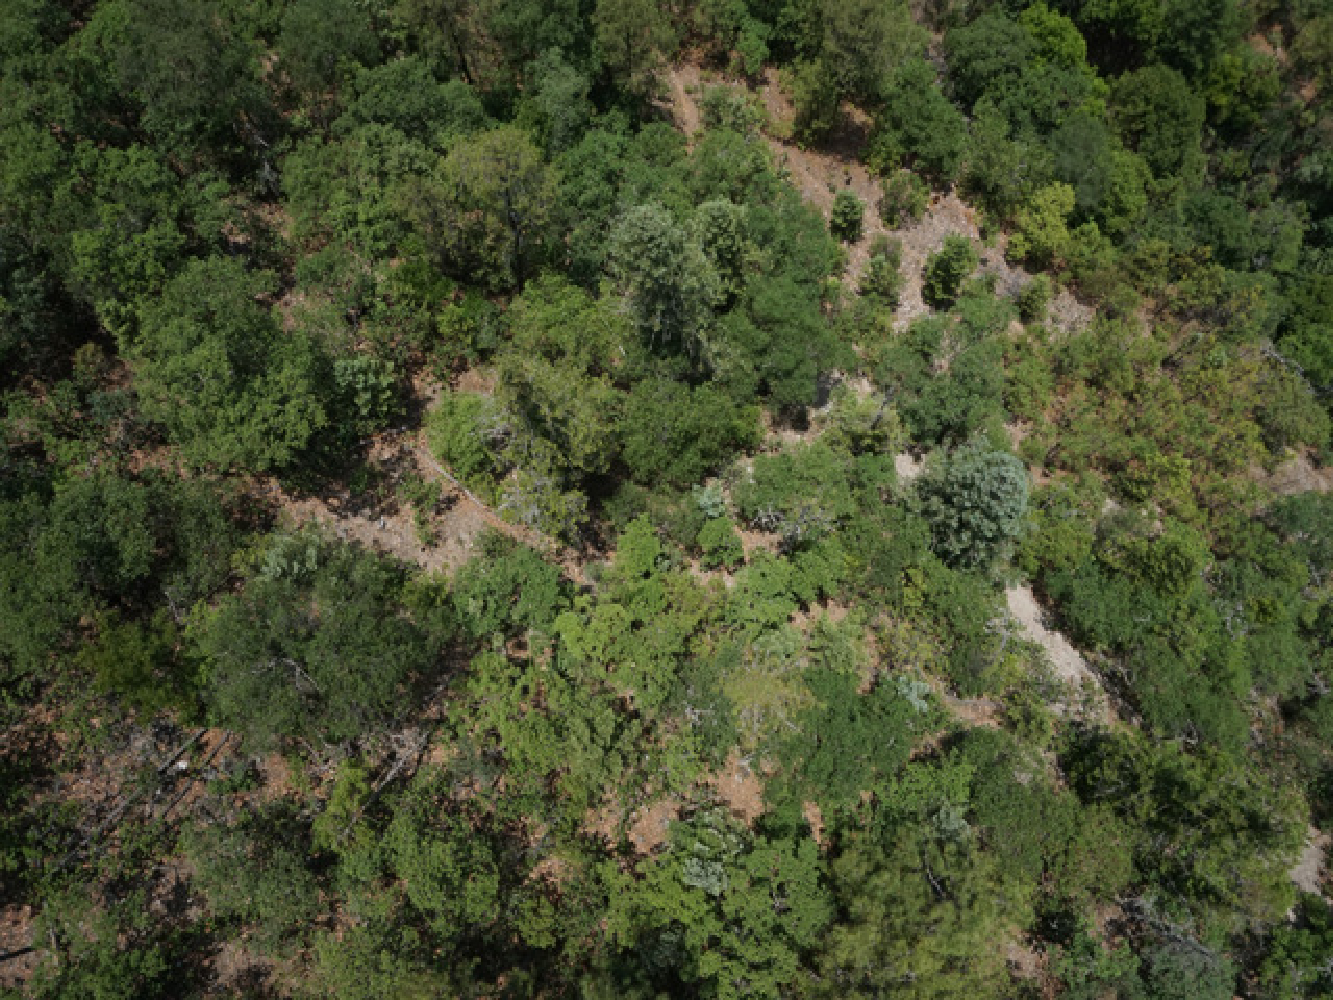
\includegraphics[width=0.45\textwidth]{DSC06100}} & 
\subfloat[Histograma generado]{\includegraphics[width=0.45\textwidth]{histograma-gen}} &
  \end{tabular}
  \caption[Histograma de color]{Histograma de color generado con las bibliotecas \texttt{matplotlib y OpenCV.}}
  \label{Histograma-generado}
\end{figure}

\subsubsection{Forma}
La característica de forma cuenta también con varias métricas, se hace énfasis en los \emph{momentos de una imagen}. Los momentos de una imagen son los pesos promedio de la intensidad de píxel sobre una imagen.

\begin{figure}[h!]
  \centering
    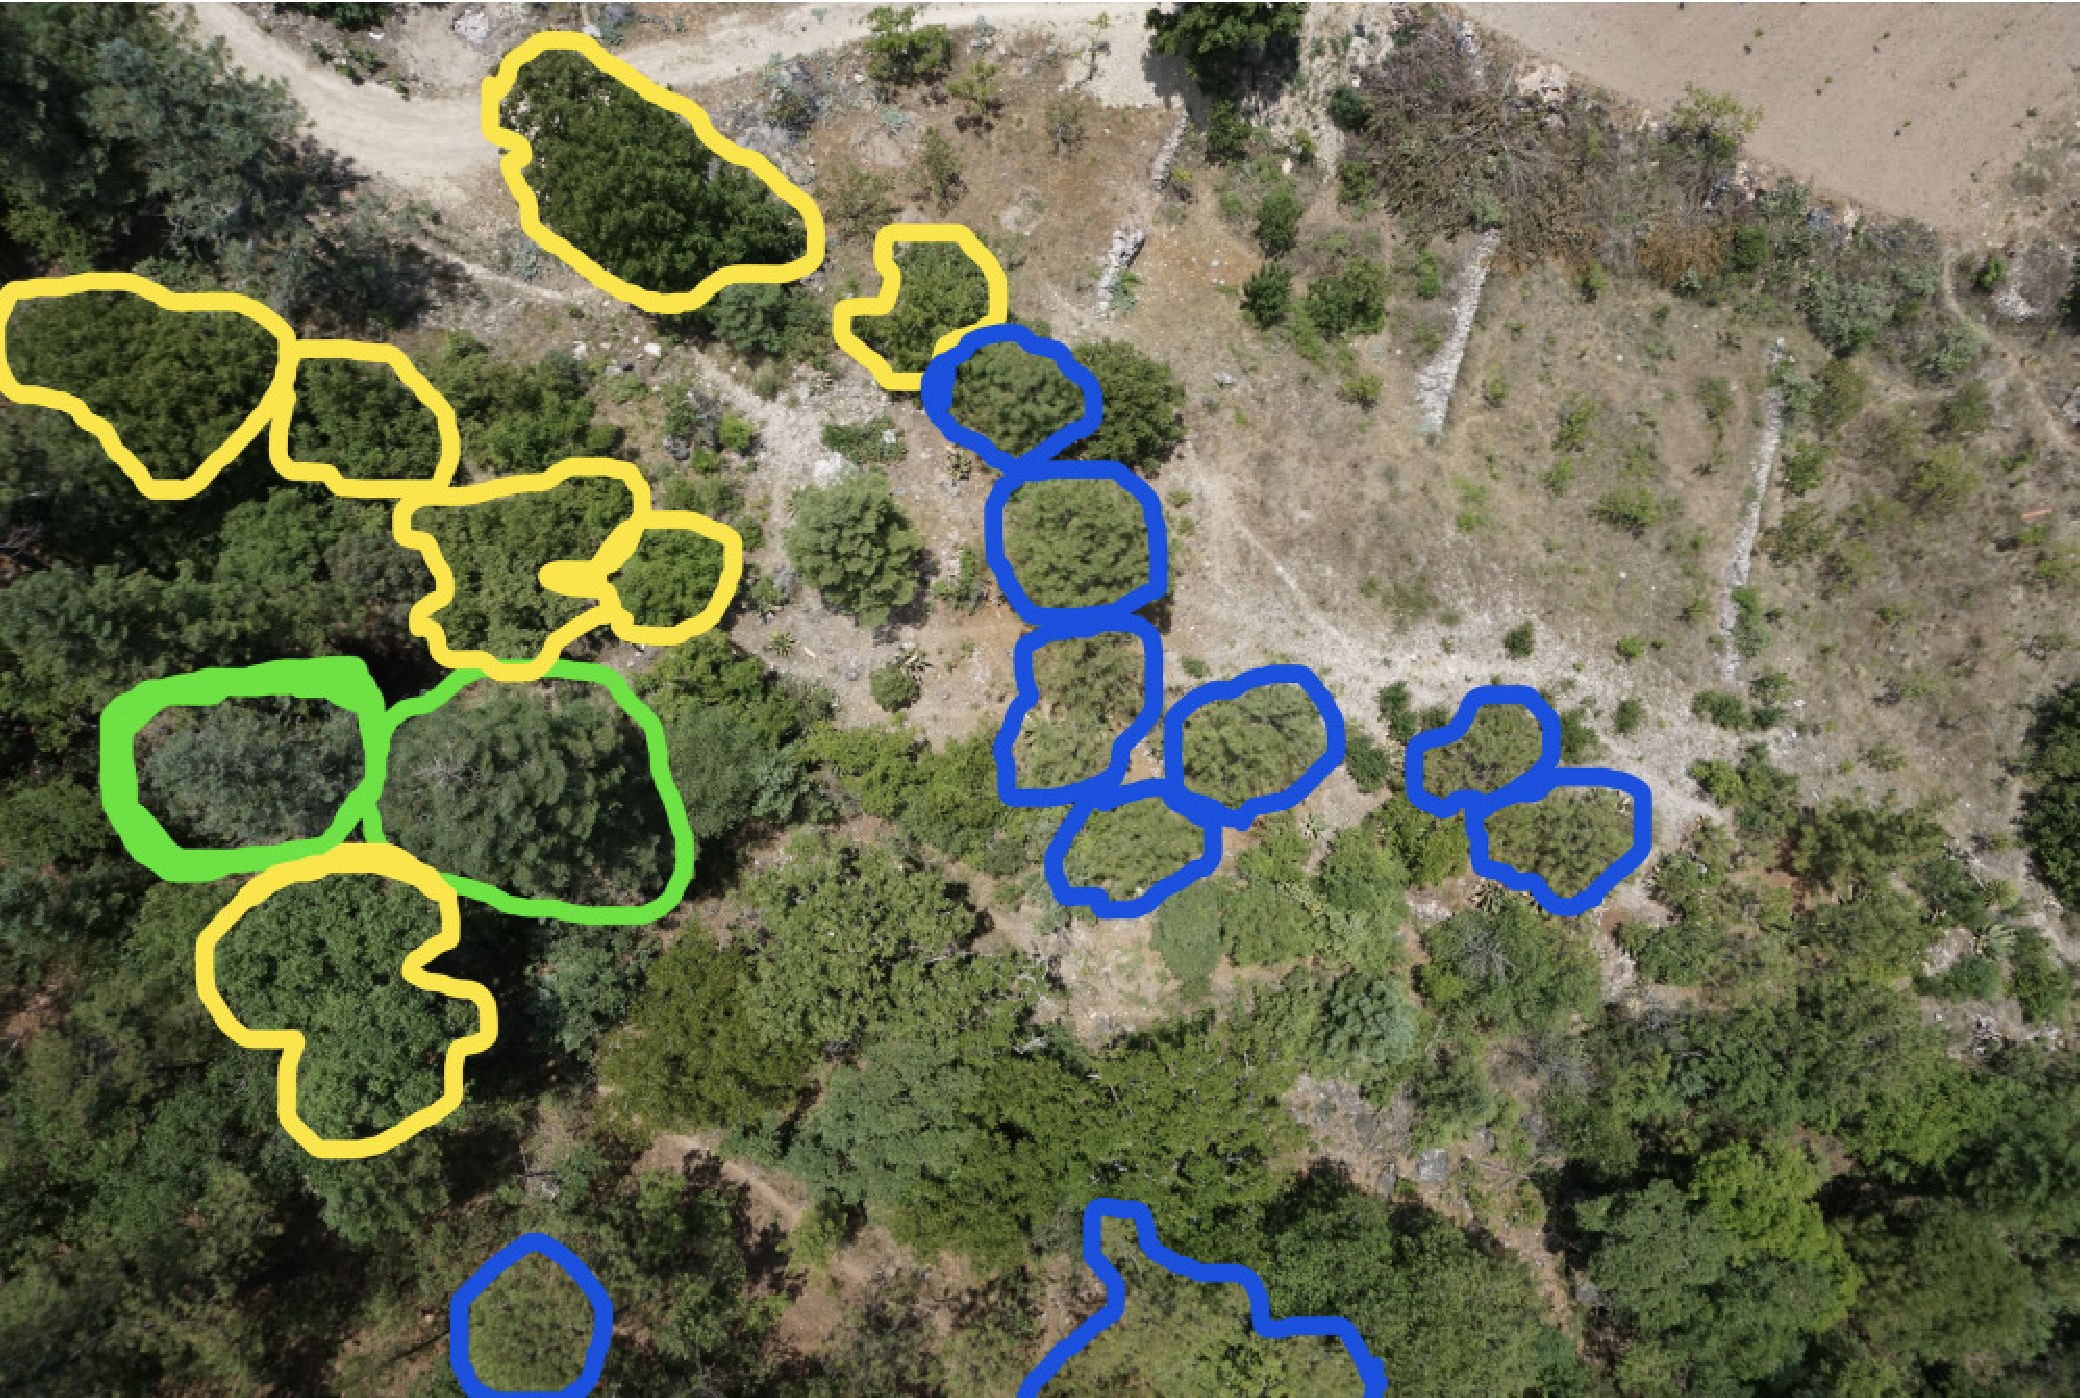
\includegraphics[width=0.45\textwidth]{Anotaciones-ex}
    \caption[Formas de cada especie arbórea.]{Formas de cada especie arbórea (verde: Abies, azúl: Pino, amarillo: Encino).}
\end{figure}

\clearpage

\subsubsection{Textura}
Esta característica tiene una gran relevancia dado que es de las más usadas al momento de identificar objetos en regiones de interés en fotografías aéreas, micrográficas y de satélite y en el presente trabajo, al identificar las muestras de los árboles. En este caso se emplea la métrica de \emph{textura de Haralick}.\\

Esta métrica o conjunto de descriptores estadísticos de textura realizada por \citep{rf16}, se utiliza como parte de un conjunto de descriptores estadísticos de textura para determinar 14 descriptores de textura haciendo uso de la matriz de concurrencia de los valores de intensidad de la imagen (COM).

\begin{figure}[h!]
  \centering
\begin{tabular}{@{}ccc@{}}
\subfloat[Encino]{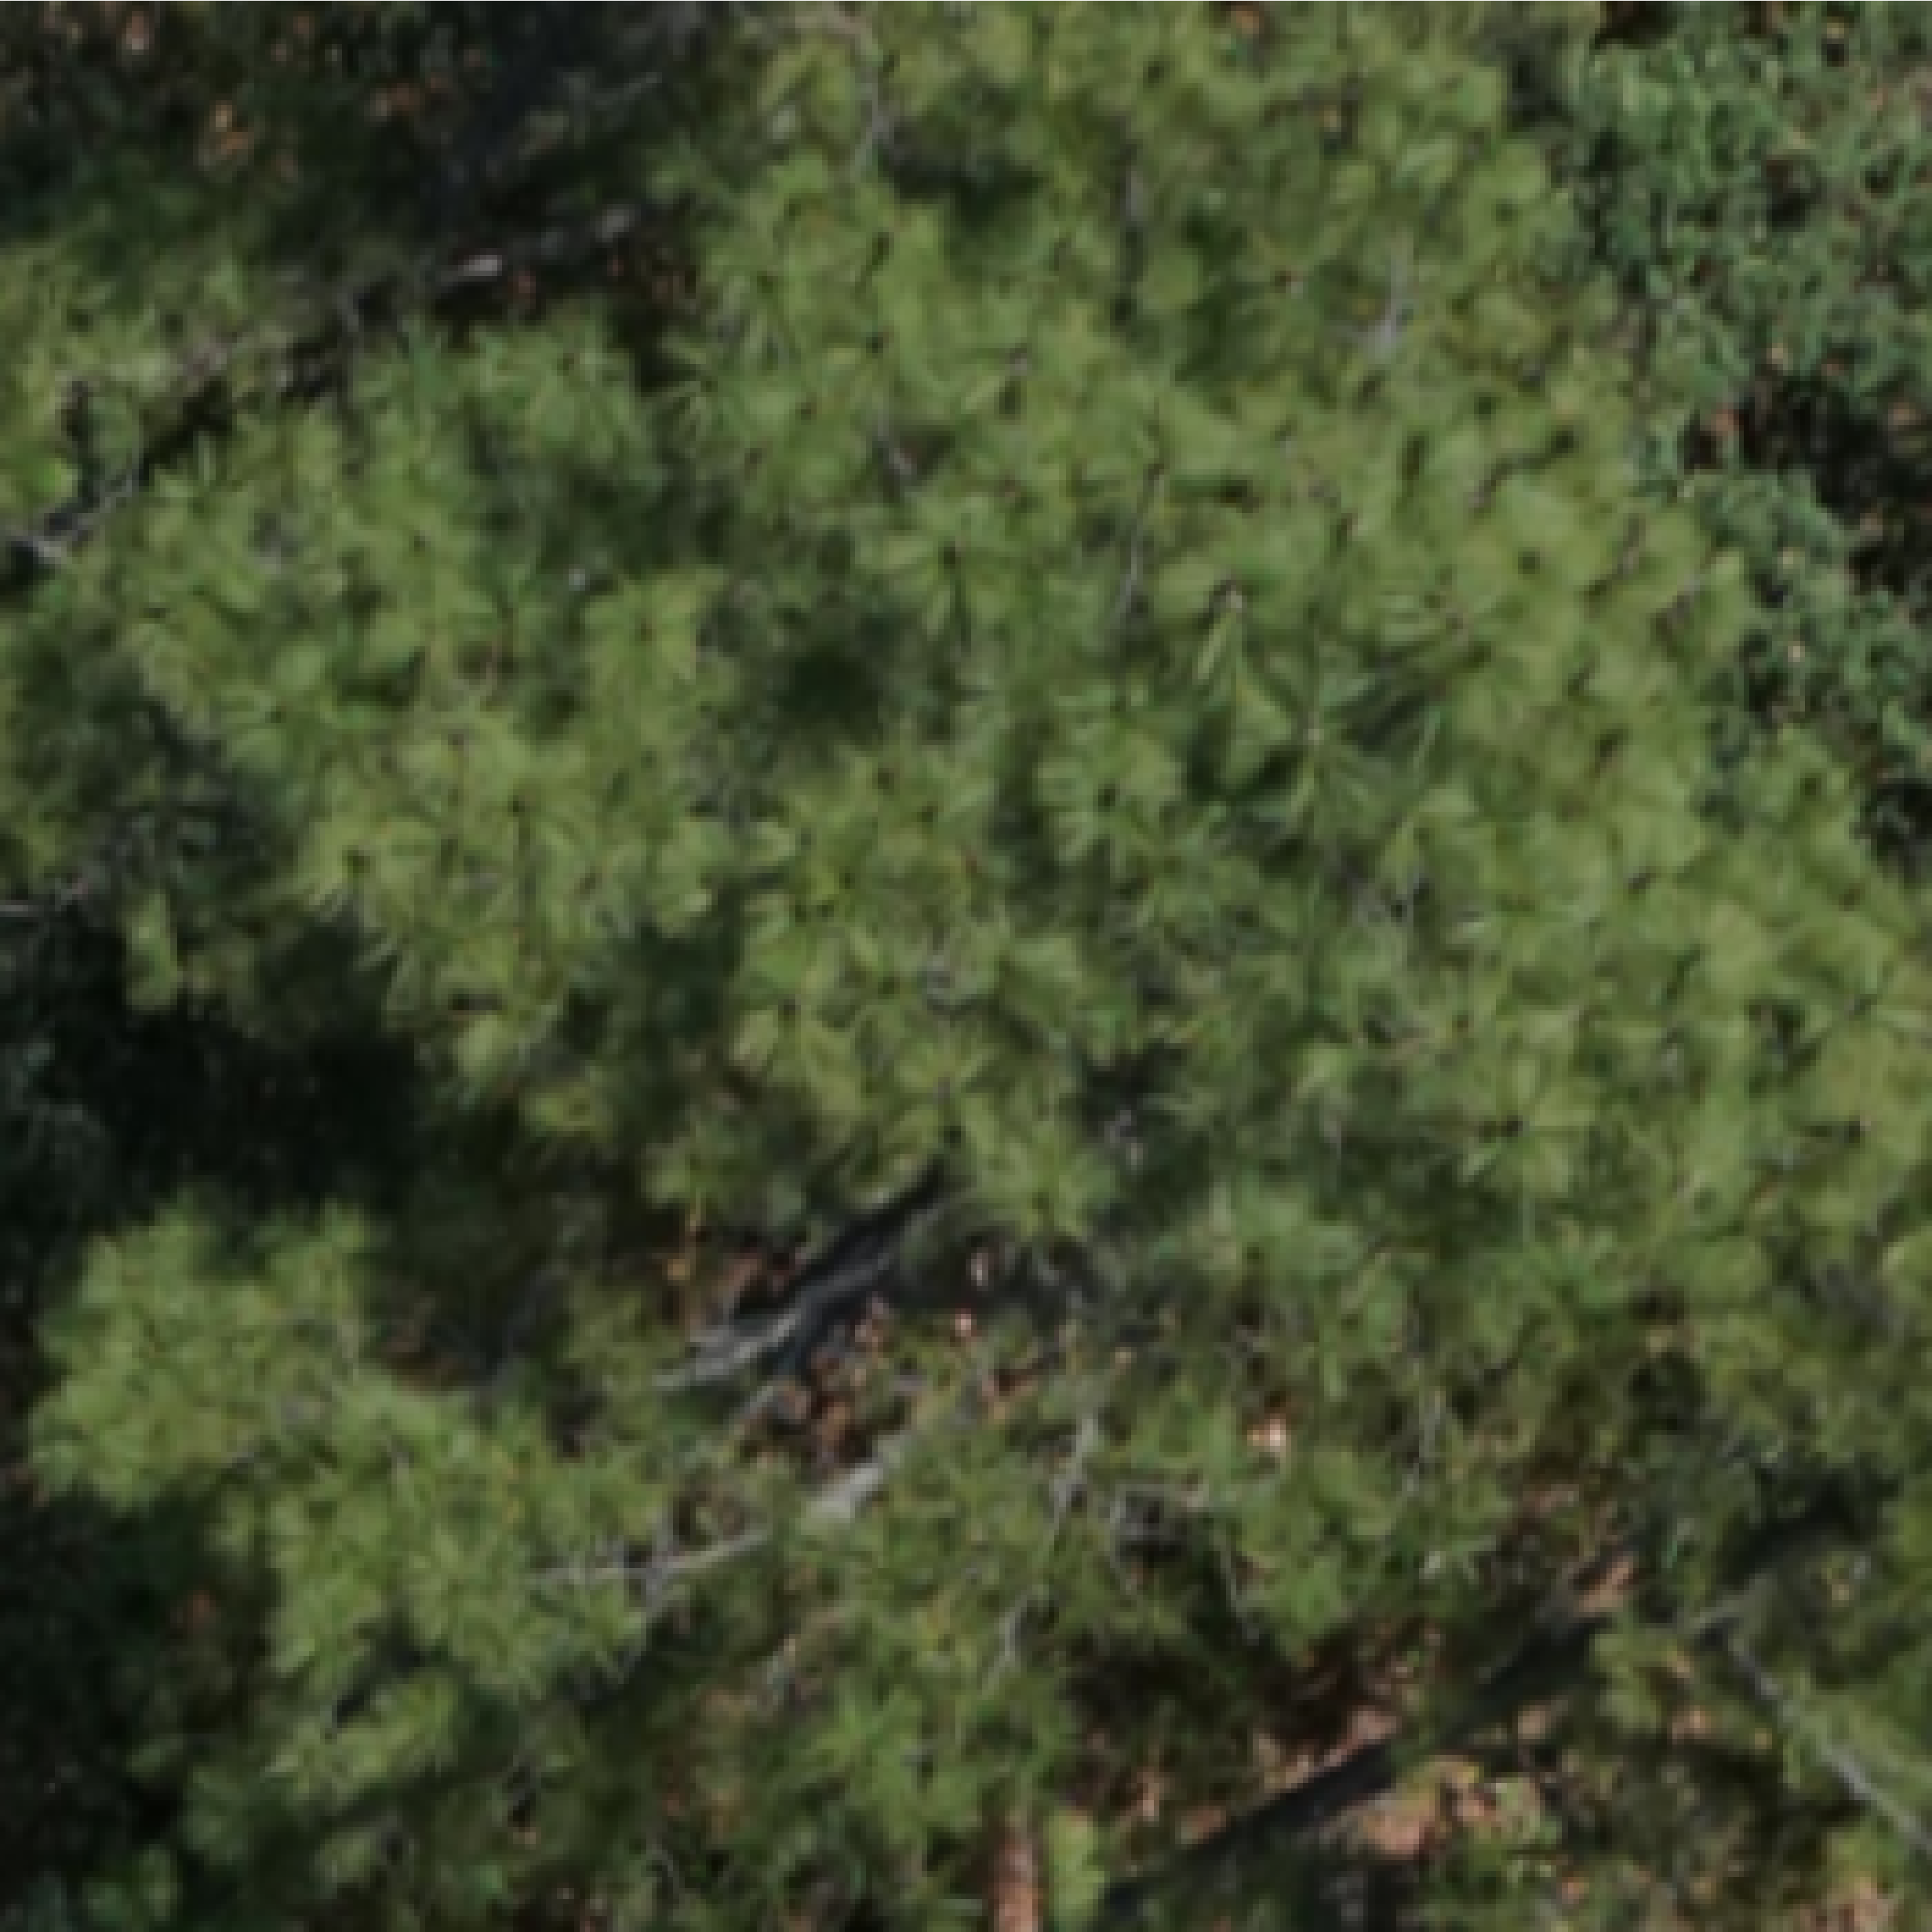
\includegraphics[width=0.3\textwidth]{1_res}} & 
\subfloat[Pino]{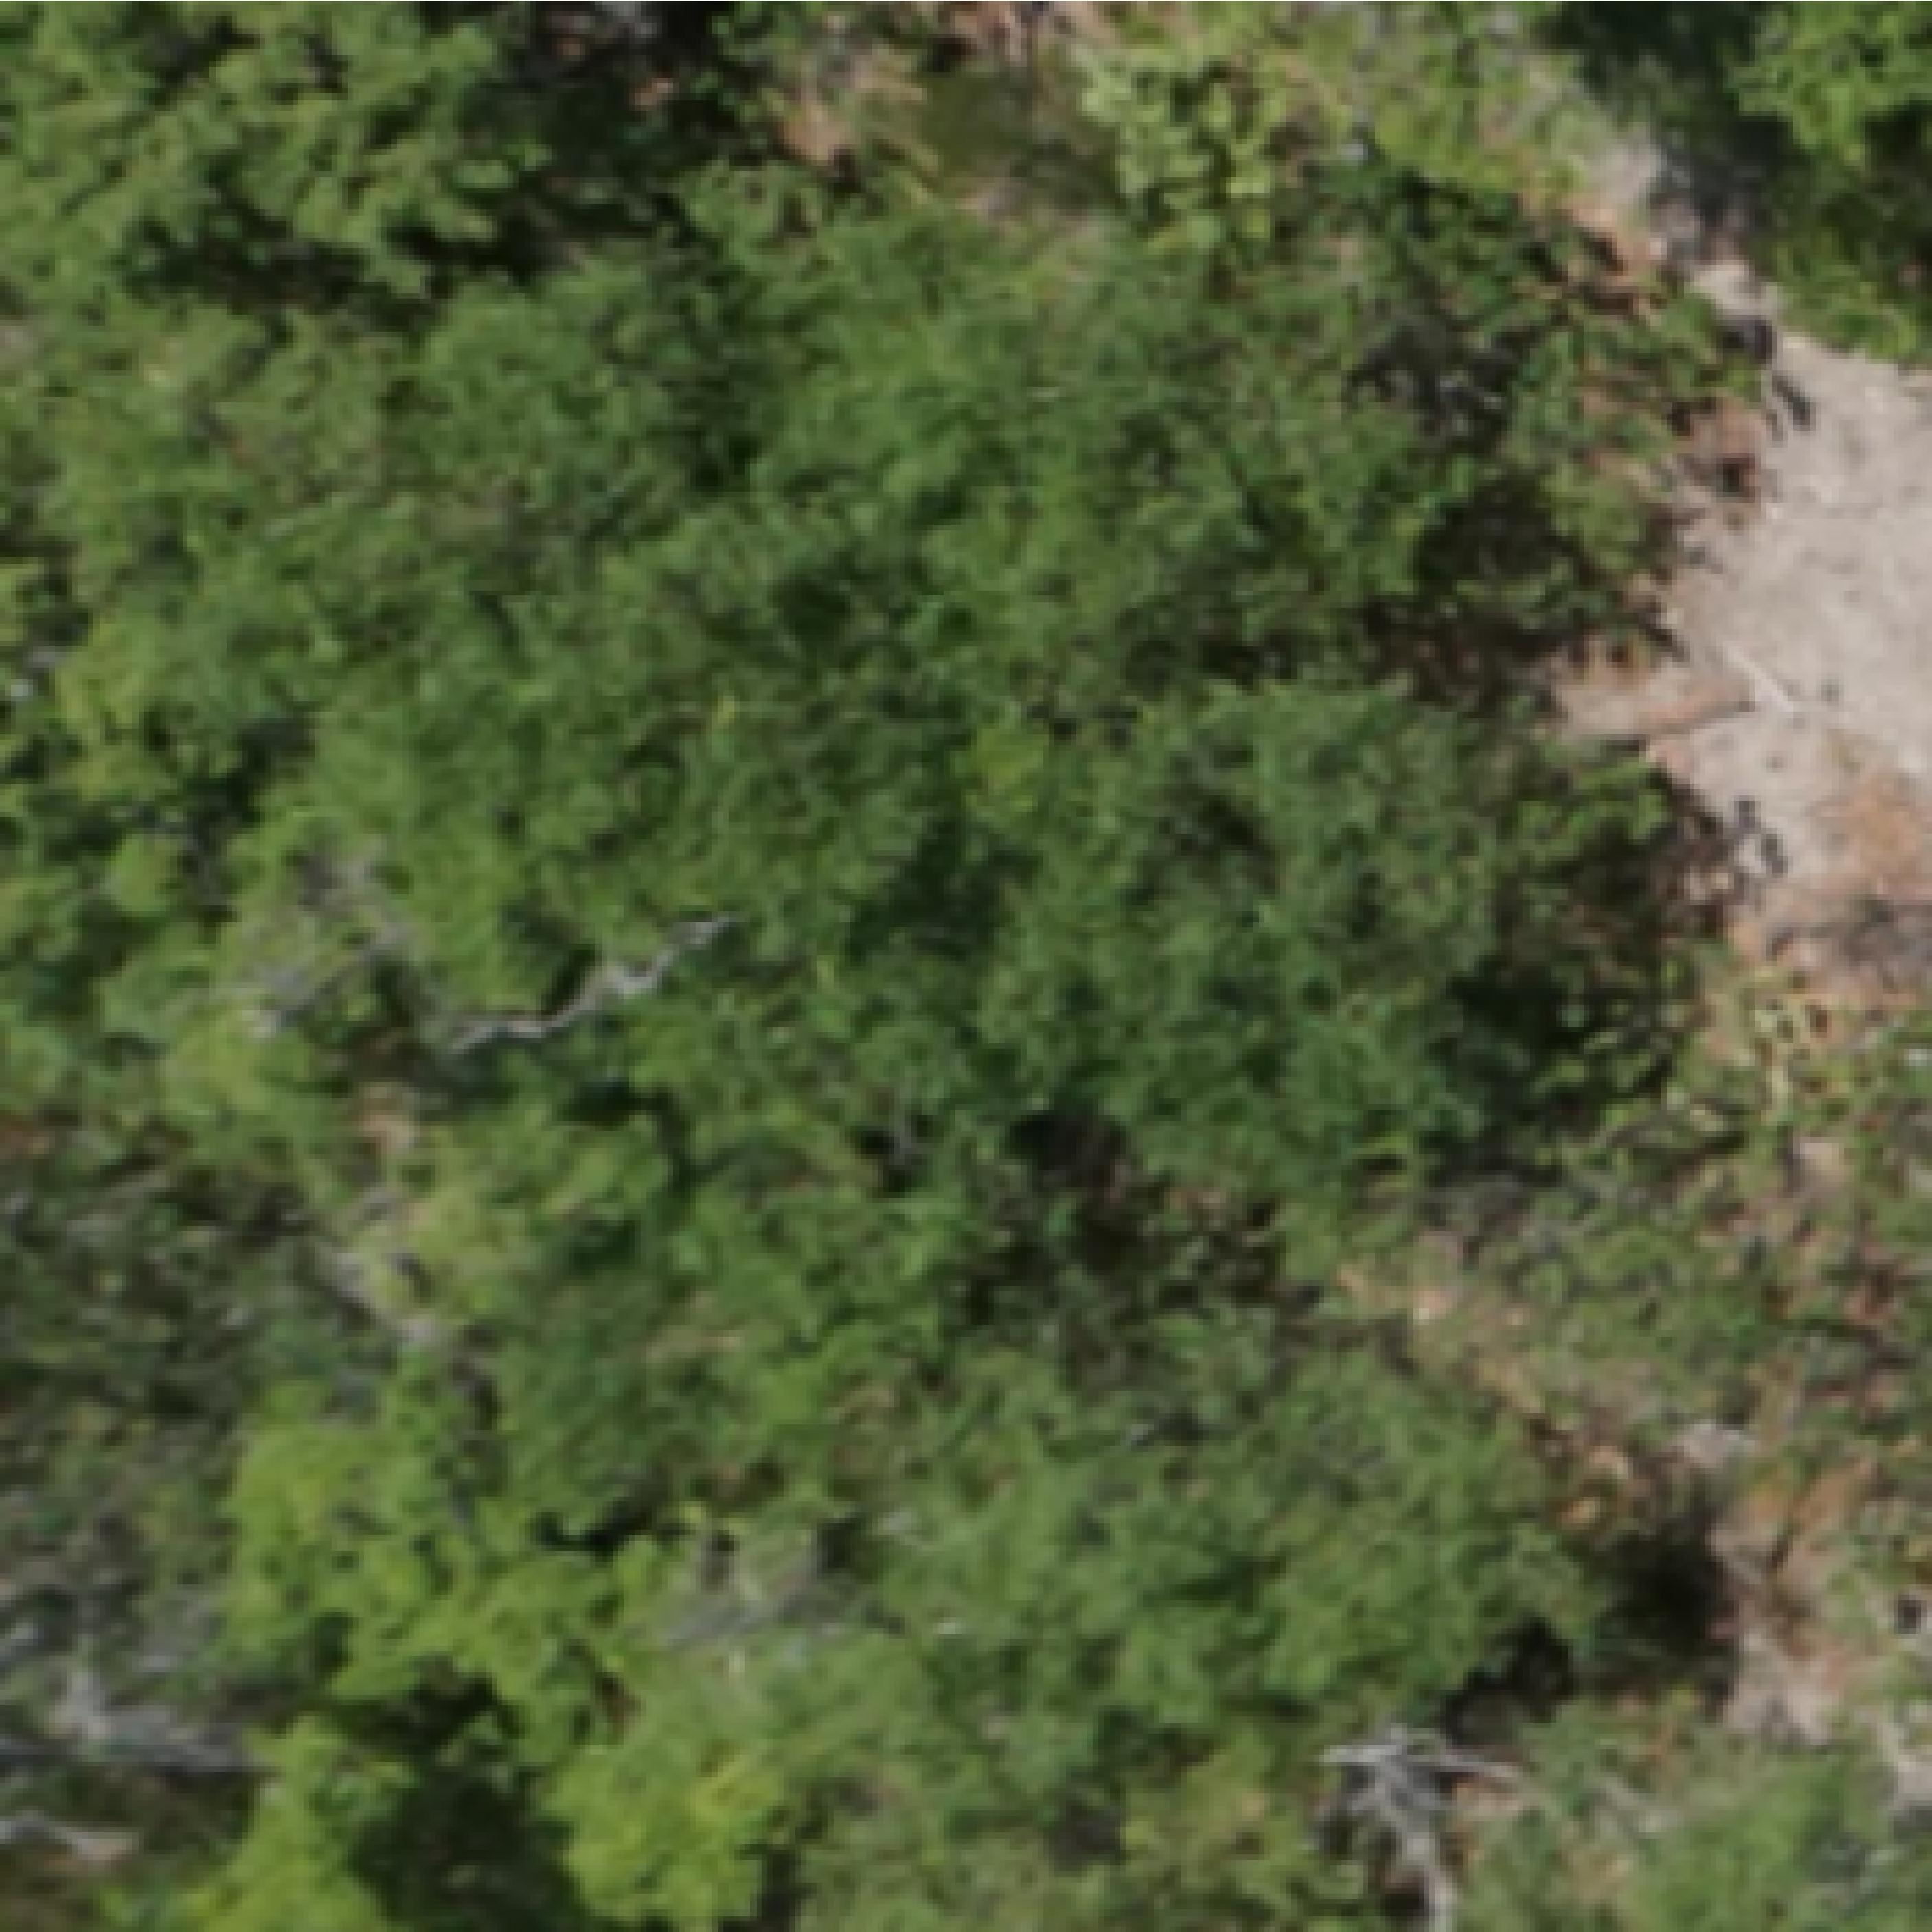
\includegraphics[width=0.3\textwidth]{2_res}} &
\subfloat[Abies]{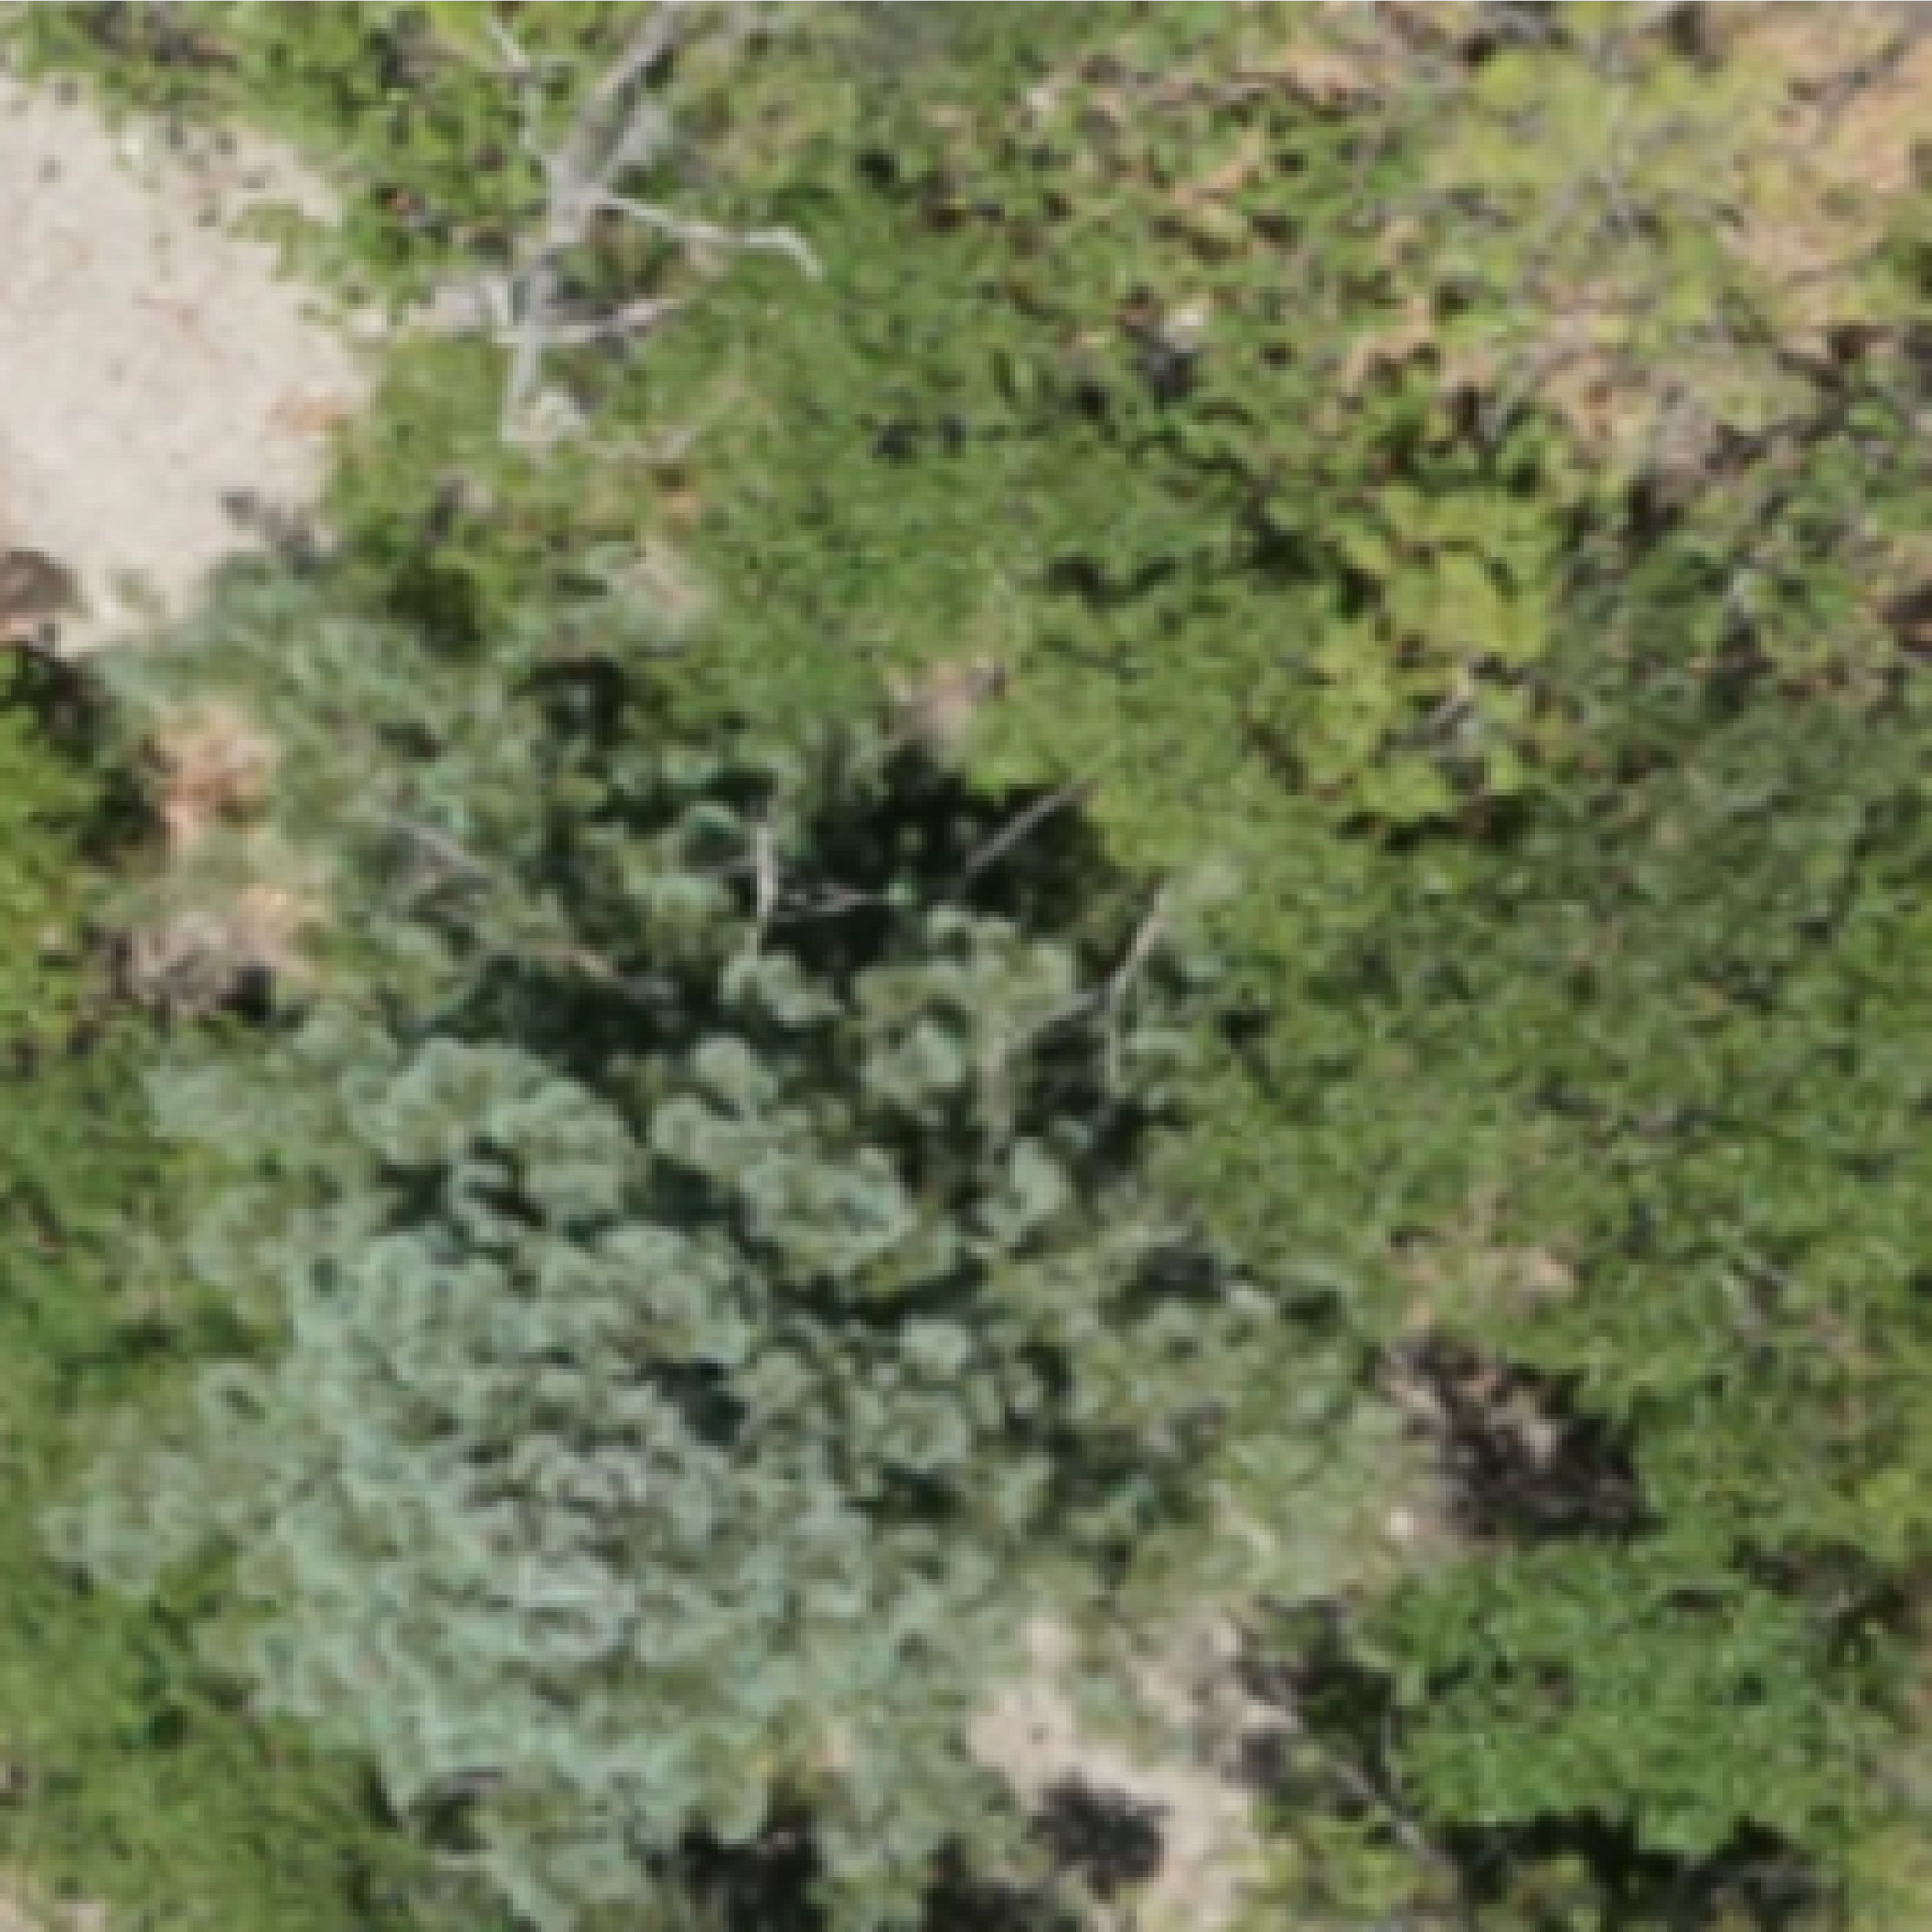
\includegraphics[width=0.3\textwidth]{3_res}}
  \end{tabular}
  \caption[Comparación de texturas.]{Comparación de texturas encontradas.}
  \label{Texturas}
\end{figure}


\subsection{Descriptores de características locales}
Como se menciono al inicio de la sección 2.2, las características locales son necesarias para describir los puntos o regiones de interés en una imagen. 

\begin{description}
\item[Escalamiento:]{Transforma los datos de las características en rangos específicos de cero a uno.}

\item[Normalización:]{Desplaza y re-escala valores para alcanzar un rango entre cero y uno.}

\item[SIFT (Característica de transformación de escala invariante)]{Extrae la información y adecua en comparaciones.}

\item[SURF (Característica de acelerado robusto)]{Toma un vecino al rededor del punto seleccionado en la imagen y es dividido en sub-regiones para cada sub-región.}

\item[BRIEF (Característica de diferencias en forma de cadena binaria)]{Se enfoca en la orientación y menor numero de diferencias a su alrededor.}

\item[ORB (BRIEF rotada y orientada rápida)]{Determina estos puntos clave de una imágen.}
\end{description}

\subsection{Uso de descriptores}
Existen varias formas de utilizar los descriptores pero hay dos maneras de mezclar las características de vectores.

\paragraph{Para las características globales de vector, sólo se concatena cada característica del vector para formar a una característica global del vector simple. Este enfoque se utiliza en el desarrollo de este algoritmo} 

\paragraph{Para las características locales del vector también puede hacerse una combinación de las características locales y globales del vector, es necesario algo llamado \emph{modelo de la bolsa de palabras} (BOVW). Este enfoque se utiliza normalmente en constructores de vocabularios, agrupamiento de $K$-medias, etc} 

\section{Trabajos relacionados}
Existen algunos trabajos que no están completamente relacionados con el objetivo de identificar especies arbóreas, pero si existen investigaciones que toman como objetivo el analizar zonas forestales.\\

\citet{rf14} menciona como hacen uso de combinar datos para realizar inventarios forestales por medio de sistemas digitales aéreos de fotogrametría y escáneres láser.\\

\citet{rf1}  utilizan una gran cantidad de entradas para definir manualmente la especie utilizando técnicas tradicionales.\\
 
\citet{rf2} tienen como meta evaluar artículos para actualizar los inventarios de árboles en un área metropolitana.\\ 

\citet{rf3} tienen como objetivo detectar objetos además de hacer uso del umbral adaptativo, el cual es muy utilizado en la visión computacional.\\

\citet{rf9} hace simulaciones para la gestión de modelos forestales que podría ser requeridos para la toma de decisiones en un sector forestal.\\

\citet{rf10} hacen uso de técnicas de inteligencia artificial para la identificación  de especies forestales haciendo uso de multidatos espectrales tomando como punto de partida, los vecinos más cercanos (KNN).\\
\vspace*{-4mm}
\begin{table}[h!]
\centering
\caption{Comparación de trabajos frente al desarrollado, donde \checkmark indica que cumple con esta característica y  $\times$ no cumple con esta característica.}
\begin{adjustbox}{width=0.35\textwidth}
\begin{tabular}{|l|c|c|c|}
\hline
Trabajo & \rotatebox[origin=c]{90}{Inventarios forestales}& \rotatebox[origin=c]{90}{Visión computacional} & \rotatebox[origin=c]{90}{ Detección de objetos}\\
	\hline
    \citet{rf1} & \checkmark & $\times$ & \checkmark\\
    \hline
    \citet{rf2}&  \checkmark  &  $\times$ & $\times$ \\
    \hline
    \citet{rf3}& $\times$ & \checkmark & \checkmark\\
    \hline
    \citet{rf9}& \checkmark & \checkmark & \checkmark\\
	\hline    
    \citet{rf10}& $\times$ & \checkmark & \checkmark\\
	\hline    
    \citet{rf11}& $\times$ & \checkmark & \checkmark\\
	\hline    
    \citet{rf12}& \checkmark  & $\times$ & $\times$\\
	\hline    
    \citet{rf13}& \checkmark & $\times$ & $\times$\\
	\hline    
    \citet{rf14}&  $\times$ & \checkmark & $\times$\\
	\hline    
    \citet{rf15}& \checkmark & \checkmark & $\times$\\
	\hline    
    El presente trabajo & \checkmark & \checkmark & \checkmark\\
    \hline
\end{tabular}
\end{adjustbox}
\label{tab:Comparación de trabajos frente al desarrollado}
\end{table}
\clearpage

\subsection{Áreas de oportunidad}
En el método propuesto la visión computacional hace uso del modelo generado previamente por el aprendizaje máquina, el cual se encarga de clasificar cada árbol mediante una etiqueta que define a su especie por color. Esto último no ha sido aplicado en las investigaciones encontradas puesto que tienen un enfoque en hacer clasificaciones de múltiples objetos de un sólo tipo, o bien, sólo se enfocan en hacer anotaciones manuales por medio de inputs previamente establecidos y esto únicamente se enfoca en comparaciones.\\

En el cuadro \ref{tab:Comparación de trabajos frente al desarrollado} se puede apreciar que características comparte el trabajo desarrollado con el de otros autores. También se puede percibir que otros trabajos tengan las mismas características o al menos casi todas de las que tiene el trabajo desarrollado, sin embargo, el presente trabajo además de generar un inventario forestal de forma automatizada, el código fuente del trabajo puede ser modificado o estudiado con otros propósitos sin necesidad de esperar una retribución de por medio debido a que es un software libre.

\section{Solución propuesta}
La solución propuesta se va a divir en siete fases, en dicha solución se parte de la recolección de muestras y finaliza en la generación de un inventario forestal con muestras detectadas por medio del aprendizaje máquina y la visión computacional.

\subsection{Fase de recolección de muestras}
La primera fase en el desarrollo de la solución consiste en recolectar muestras de el objeto a identificar por medio del aprendizaje máquina. 

\subsubsection{Muestras recolectadas}
Inicialmente se empezó descargando el repositorio con imágenes que contenía imágenes de las zonas donde se realizó el recorrido del dron, más específicamente \emph{Cilantrillo} y \emph{Trinidad}.

\subsubsection{Análisis de muestras}
La información de cada muestra es analizada píxel por píxel, por lo que a simple vista se puede percibir la clase de información que contiene cada muestra, pero el analizar cada una de ellas llevaría demasiado tiempo, por lo que, se puede concluir que hay píxeles dentro de ellas que no sean útiles. En la figura \ref{Comparación de muestras} se muestra un ejemplo de cómo se verían las muestras que son de utilidad.

\begin{figure}[h!]
  \centering
\begin{tabular}{@{}ccc@{}}
\subfloat[Muestra no útil]{\includegraphics[width=0.48\textwidth]{DSC06080}} & 
\subfloat[Muestra útil]{\includegraphics[width=0.48\textwidth]{DSC06080-sf-2}} &
  \end{tabular}
  \caption[Comparación de muestras]{Comparación de muestras donde se aprecia una útil de una no útil.}
  \label{Comparación de muestras}
\end{figure}

\subsubsection{Información no útil}
En cada una de las muestras recolectadas está presente el suelo ya que es una imagen capturada por un drone, sin embargo, el suelo forma parte de la información que se necesita remover de las muestras para no sobre entrenar a el modelo de reconocimiento previamente desarrollado.\\

Para remover este suelo, se convierte la muestra a formato \texttt{png} con canales  RGBA (rojo, verde, azúl y transparencia, siglas en inglés), una vez que la muestra tenga el canal transparente, se recorren todos los píxeles de la imagen con el fin de encontrar y descartar los píxeles que no tengan relación con los colores de los árboles y así sólo guardar muestras con la información útil como se muestra en la figura \ref{Comparación de muestras} (b).

\subsection{Fase de procesamiento de muestras}
Una vez recolectadas las muestras con información relevante, se procede a  entrenar a el modelo con esa información para que sea en fases posteriores este sea capaz de entender y clasificar donde estén presentes las especies arbóreas almacenadas en el modelo.

\subsubsection{Recortando muestras}
Primeramente hay reconocer las secciones o partes de la muestra que son de interés, en este caso, se trabaja con los colores, específicamente los de cada especie de árbol. En todas las muestras, se tienen tres colores: [verde, amarillo, azul]. Estos colores indican que colores tienen una anotación válida para recortar.

\begin{figure}[H]
  \centering
      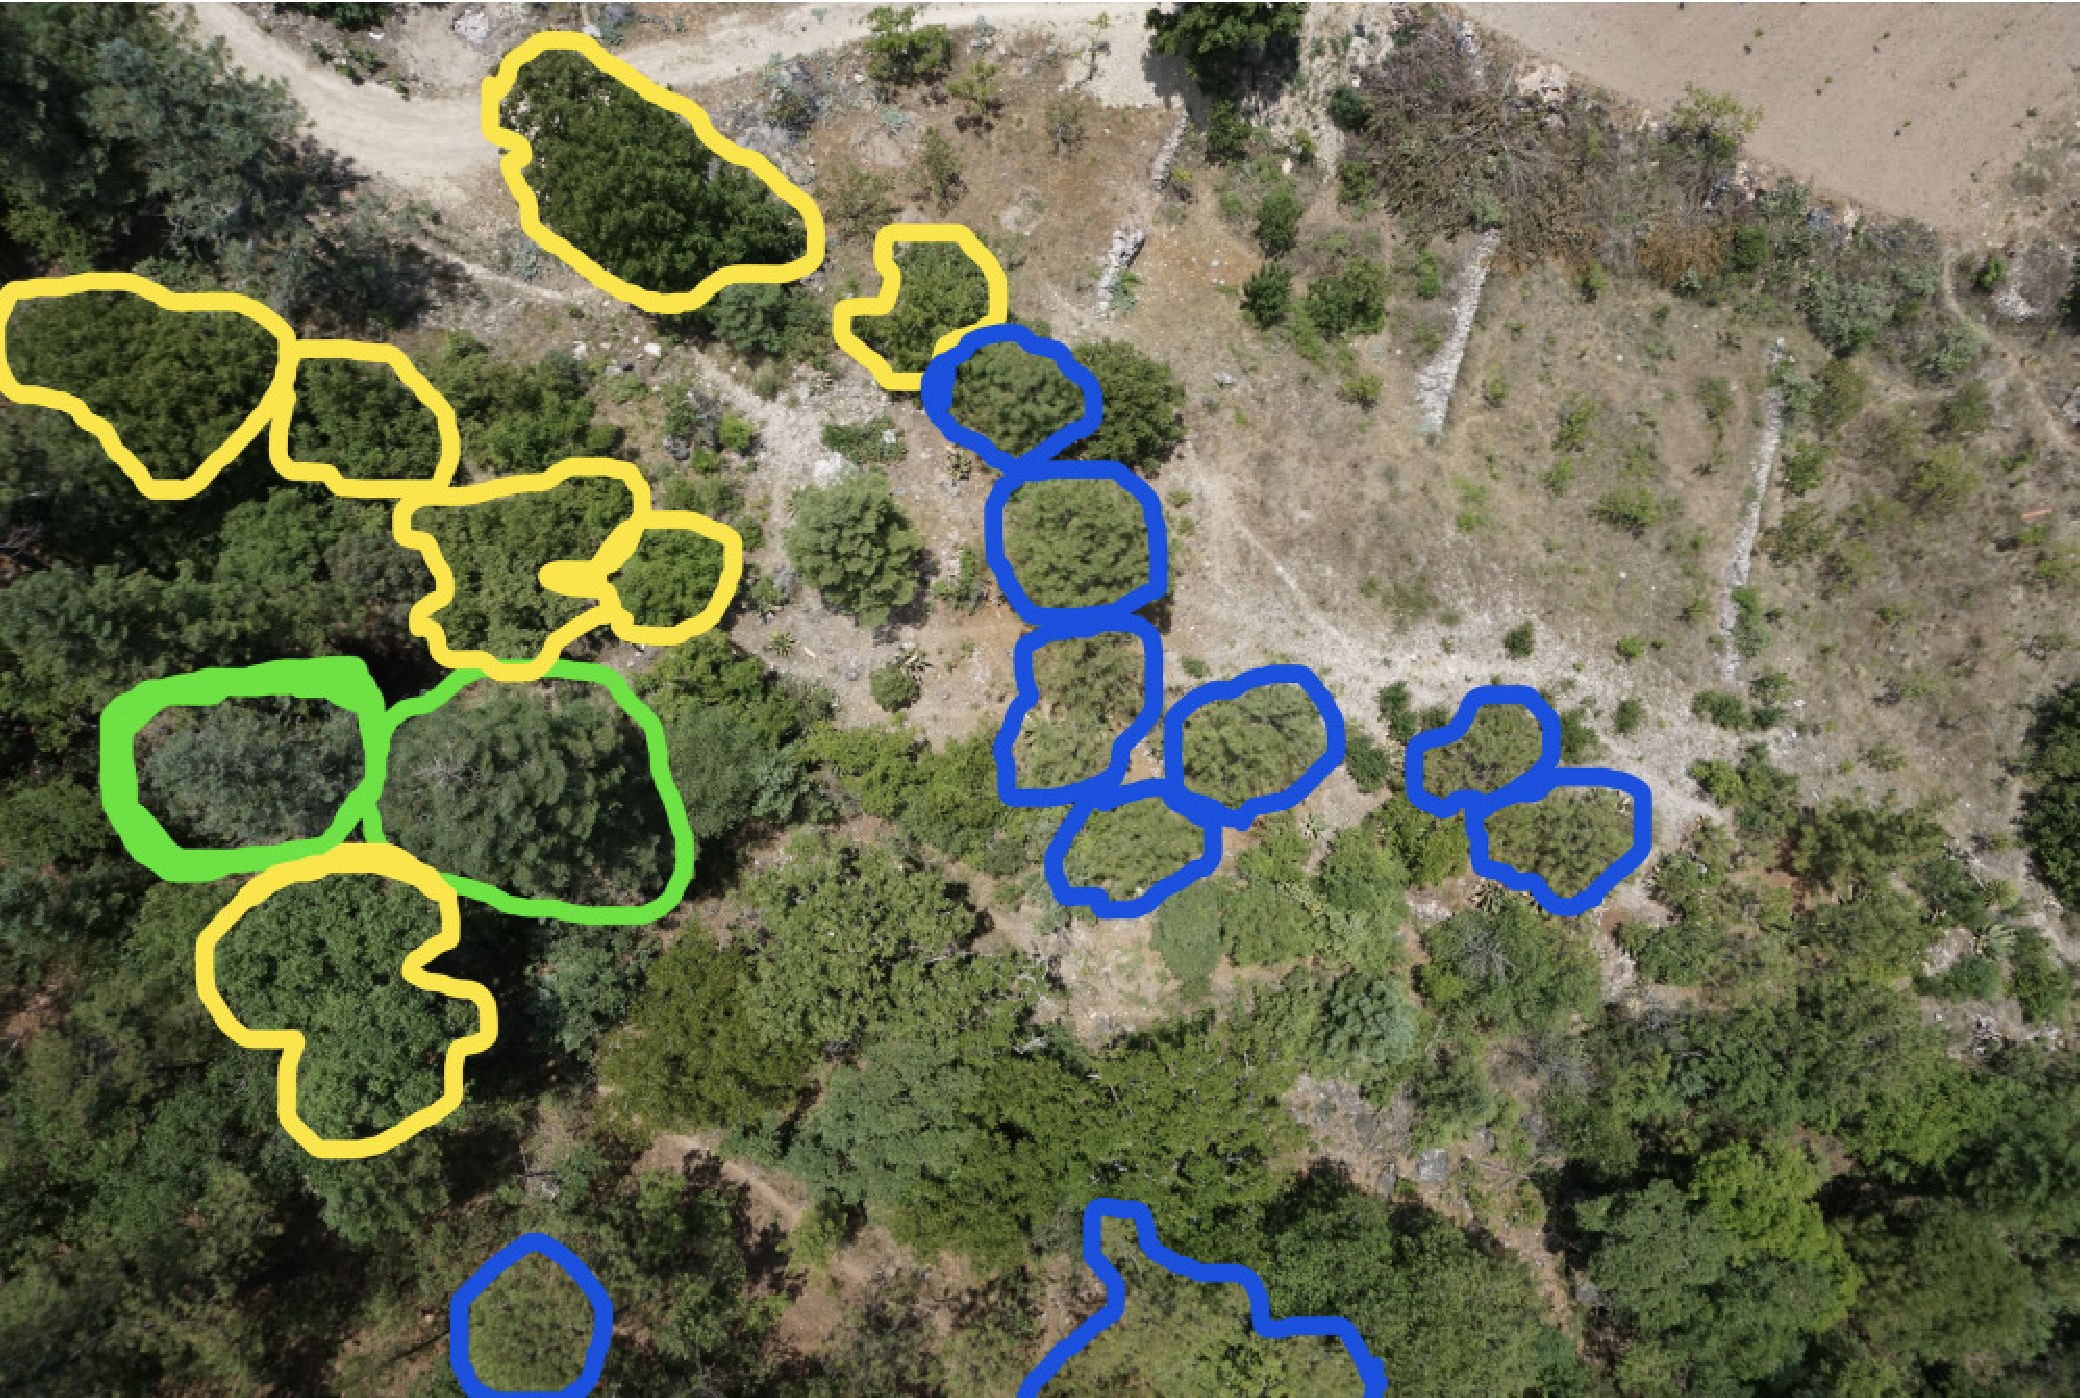
\includegraphics[width=0.50\textwidth]{Anotaciones-ex}
    \caption{Muestra con anotaciones}
    \label{Muestra con anotaciones}
\end{figure}

En la figura \ref{Muestra con anotaciones} se aprecia que tiene secciones delimitadas por colores, por lo que se recorre la muestra por píxeles hasta encontrar la zona que esté dentro del rango de colores previamente establecido.

\subsection{Fase de entrenamiento}
Previo a la detección de especies en las muestras se genera el modelo encargado de clasificar las muestras, para esto, el algoritmo necesita saber que imágenes o carpetas de imágenes tomará en cuenta para analizar la información que va a estar presente en el modelo de información de especies de arboles. 

\subsection{Fase de detección}
En esta fase se utilizan las características globales y el modelo clasificador de {\em bosque aleatorio}\footnote{Clasificador de múltiples decisiones que funciona en conjunto.} (inglés: random forest), donde se establece un valor estimado de árboles por cada muestra donde se vaya a probar el modelo y posteriormente clasificar cada especie por color y nombre como en la figura \ref{Clasificación de especies arbóreas en una muestra}.
\\

\begin{figure}[H]
  \centering
         \includegraphics[width=0.5\textwidth]{result_new}
    \caption{Clasificación de especies arbóreas en una muestra}
    \label{Clasificación de especies arbóreas en una muestra}
\end{figure}

\subsection{Fase de combinación}
La fase de combinación consta en tomar la muestra del directorio original de imágenes, asignarlo como base y posteriormente, la muestra con información útil del directorio que se genero como resultado de la fase de detección, es incrustado encima de la muestra original para obtener un resultado como el de la figura \ref{Combinación de detección y una muestra original}.


\begin{figure}[H]
  \centering
  \includegraphics[width=0.5\textwidth]{result_combination}
    \caption{Combinación de detección y una muestra original}
    \label{Combinación de detección y una muestra original}
\end{figure}
\clearpage

\section{Evaluación}
Después de clasificar todas las muestras que pasan por las fases de entrenamiento, detección y combinación, se puede obtener un resultado preliminar que indica  cuántos árboles de cada especie son detectados en la fase de detección. El analizar una muestra que haya pasado por la fase de combinación puede evaluar si los parámetros seleccionados dan un resultado favorable o si estos podrían mejorar cambiando alguno de ellos, sin embargo, es experimentando como se puede determinar si es posible mejorar el resultado obtenido.\\

\begin{description}
\item[Experimento $A$: Misma cantidad de especies por tamaño de clase.]{Toma la misma cantidad de muestras para cada clase.}

\item[Experimento $B$:  Cantidad total de especies por tamaño de clase.]{Toma todas las especies disponibles en cada clase.}

\item[Experimento $C$: Misma cantidad de especies utilizando espejos de muestras.]{Utiliza espejos de las muestras recolectadas en las clases que tengan una cantidad de muestras inferior al de la clase con más muestras para tener el mismo tamaño de muestras en todas las clases.}

\item[Experimento $D$: Umbralización.]{Compara tres niveles distintos de umbral  (0.15\%, 0.25\%, 0.50\%) para comparar el que mejor resultados proporciona.} 

\item[Experimento $E$: Límite de píxeles ausentes.]{Utiliza tres porcentajes de píxeles ausentes (0.75\%, 0.80\% y 0.85\%) para determinar la mayor cantidad de especies posibles en una muestra.}
\end{description}
\clearpage

Todos los experimentos son ejecutados en una laptop con las especificaciones del cuadro \ref{tab:Especificaciones técnicas del PC}.

\begin{table}[H]
	{\centering
		\caption{Especificaciones técnicas del equipo de cómputo}
		\begin{tabular}{|c|c|c|}
			\hline
			Sistema Operativo & Windows 10 64 bits\\
			\hline
			Procesador & Intel Core i5-7300HQ\\
			\hline
			RAM & 8 GB RAM DDR4 2133 MHz\\
			\hline
		\end{tabular}

	\label{tab:Especificaciones técnicas del PC}
	}
\end{table}

Los resultados  del cuadro \ref{Resultados-obtenidos} reportan las especies detectadas por cada experimento realizado.

\begin{table}[h!]
\caption{Resultados obtenidos por experimento.}
\centering
\begin{tabular}{|c|c|c|c|}
			\hline
			 \textbf{Experimento} & \textbf{Pino} & \textbf{Encino} & \textbf{Abies}\\
			\hline
			Experimento A & 67.3 & 18.4 & 14.4\\
			\hline
			Experimento B & 50.2 & 41.6 & 8.2\\
			\hline
			Experimento C & 58.1 & 34.3 & 7.7\\
			\hline
			Experimento D (0.75) & 66 & 17 & 17\\
			\hline
			Experimento D (0.80) & 62 & 24 & 14\\
			\hline
			Experimento D (0.85) & 18 & 15 & 18\\
			\hline
			Experimento E (0.75) & 70 & 20 & 10\\
			\hline
			Experimento E (0.80) & 63 & 25 & 12\\
			\hline
			Experimento E (0.85) & 66 & 22 & 12\\
			\hline
		\end{tabular}
		\label{Resultados-obtenidos}
\end{table}

En el experimento $A$ (misma cantidad de especies por clase), Pino es claramente un especie predominante debido a que esta especie era predominante en las muestras. Como dato adicional, el experimento se completa en 18 horas.\\

En el experimento $B$ (cantidad total de especies por tamaño de clase) se aprecia que si afecta bastante fijar el tamaño de cada clase, es posible diferenciar que la especie pino ya no es tan predominante como lo era en un experimento con un valor fijo.

El experimento $C$ (misma cantidad de especies utilizando espejos de muestras) hace uso de la especie de árbol que mayor tiene muestras, donde comparando con el experimento $A$ y el experimento $B$ se puede ver  que tener un tamaño fijo de especies y un valor total de cada especie si impacta en el experimento.\\

En el experimento $D$ (umbralización) únicamente se toman en cuenta la cantidad de especies detectadas por porcentaje de píxeles permitidos, el experimento más equilibrado fue el de utilizar 0.50\% de píxeles permitidos, debido a que otorga un mejor rendimiento entre todas las muestras.\\

Finalmente para el experimento de $E$ (píxeles permitidos), se hace uso del modelo generado a partir de las muestras con el mejor umbral probado, donde se aprecia que el experimento con 85\% de pixeles permitidos es el que otorga mayor cantidad de especies arbóreas siendo ligeramente superior al experimento al experimento con 80\% de píxeles permitidos.\\

Respecto a la hipótesis que se plantea, se busca como objetivo particular el optimizar tiempos y costos de generar el inventario forestal por técnicas generadas por procesamiento de imágenes, en cuanto a tiempos definitivamente ahorrara en términos de duración si se consideran los tiempos de procesamiento y recolección de muestras, esto debido a que con un conjunto de datos relativamente grande, se puede obtener una solución en menos de tres días; en el apartado económico se puede considerar que esta técnica reduce muchos gastos en relación a equipos de trabajo, gastos en viajes a zonas particulares, etc. En cuanto a la parte de los objetivos, se cumplieron tanto el objetivo general que era generar un inventario forestal, así como los objetivos específicos, que abarcan desde la generación del conjunto de muestras hasta la parte de la prueba utilizando un modelo para detectar las especies.

\section{Conclusiones}
El objetivo de desarrollar el inventario forestal por medio de la visión computacional fue para que por medio del aprendizaje máquina se lea, analice y clasifique las especies detectadas a lo largo de una zona forestal. No obstante, dependerá en gran medida de los parámetros utilizados el alcance que tenga la ejecución de la solución, para efectos prácticos, en desarrollo de la tesis sugiere utilizar algunos valores con buen resultado tanto para el umbral adaptativo así como para los píxeles admitidos por muestra analizada.\\

La solución propuesta surgió a partir de un problema de clasificación de flores \citep{rf17},  donde originalmente solamente se utilizaban muestras de flores para determinar un tipo individual de flora pero gracias a la base, se modificó el planteamiento para utilizarlo en un entorno distinto al original. En este caso, utilizarlo para generar inventarios forestales donde una muestra de una zona forestal, es recortada por colores para posteriormente y almacenada en una carpeta que corresponde al color detectado de la especie arbórea. Posteriormente en cada carpeta de la especie detectada, hace un análisis de la información de la muestra para generar un modelo  o conjunto de datos que sirve para almacenar la información general de todas las muestras y sirva como base para detectar especies arbóreas en las muestras originales.\\

No obstante, esta solución, aunque es eficiente, puede ser mejorada si se encuentran mejores métodos para encontrar parámetros exactos en relación a los umbrales, tamaño de imágenes y una arquitectura de la solución que pueda aprovechar todos los recursos de la computadora para generar lo más rápido posible, un resultado. Otra de las cosas que se podría estudiar de mejor forma, sería la robustez de la solución propuesta, esto con apoyo de la recolección de más muestras, capturar muestras en distintas fechas y  utilizar distintas alturas en vuelos para obtener una mejor perspectiva de la zona forestal que se va analizar.


\bibliography{mybibfile}

\end{document}